\begin{frame}
\frametitle{Équations de Maxwell / Système de Friedrichs}
\vfill
Divergence supposée nulle au cours du temps :
\begin{align*}
	\Ptl{t} \EPrm \E + \ECnd \E - \Rot \H &= 0 ,
	\tag{Maxwell-Ampère}
	\\
	\Ptl{t} \HPrm \H + \HCnd \H + \Rot \E &= 0 .
	\tag{Maxwell-Faraday}
\end{align*}
\vfill
\begin{columns}%[c]
\column{.3\textwidth}
\column{.2\textwidth}
\begin{figure}
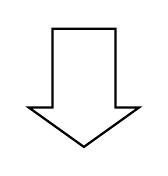
\begin{tikzpicture}[scale=0.5]
	% Fleche
	\draw[-,thick] (0,0) -- (1.4,1) -- (0.8,1) -- (0.8,3) -- (-0.8,3) -- (-0.8,1) -- (-1.4,1) -- cycle;
\end{tikzpicture}
\end{figure}
\column{.3\textwidth}
\begin{align*}
\W &= 
\begin{pmatrix}
	\E(\x,t) \\
	\H(\x,t)
\end{pmatrix}
\in \EnsR^6 ,
\\
\NC &= \dim(\EnsR^6) = 6 .
\end{align*}
\column{.2\textwidth}
\end{columns}
\vfill
\begin{align*}
	\Ptl{t} \At \W + \ACnd \W + \sum_{i=1}^3 \Aidi \W = 0 .
	\tag{Système de Friedrichs}
\end{align*}
\vfill
\begin{itemize}
\item Matrices symétriques, $\At$ définie positive et $\ACnd$ positive ;
\item Nous considérons le problème sans sources ($\ACnd = 0$).
\end{itemize}
\begin{block}{Notation d'Einstein}
Dans la suite nous utilisons la convention de sommation des indices répétés,
\textit{i.e.} $\sum_{i=1}^3 \Aidi = \Aidi$.
\end{block}
\vfill
\end{frame}

